\documentclass[Journal, InsideFigs, DoubleSpace]{ascelike} %NewProceedings, Journal

%include package for inserting picture
\usepackage{graphicx}%insert image
\DeclareGraphicsExtensions{.pdf,.png,.jpg}
\graphicspath{{figures/}}%folder contains images

\usepackage{caption}%packages for inserting multiple pictures
\usepackage{subcaption}%packages for inserting multiple pictures

\usepackage{array}%for table with fixed width
\newcolumntype{L}[1]{>{\raggedright\let\newline\\\arraybackslash\hspace{0pt}}m{#1}}
\newcolumntype{C}[1]{>{\centering\let\newline\\\arraybackslash\hspace{0pt}}m{#1}}
\newcolumntype{R}[1]{>{\raggedleft\let\newline\\\arraybackslash\hspace{0pt}}m{#1}}

\usepackage{amsmath} %math package

\usepackage{algorithm} %algorithm package
\usepackage[noend]{algpseudocode} % pseudo code package

\usepackage[utf8]{inputenc}%french accents
\usepackage[T1]{fontenc} %for accented characters

\usepackage{booktabs}%allowing drawing hline in table crossing only some columns


\begin{document}

\title{InfraLex: An automatically generated lexicon to support natural language based partial model retrieval for infrastructure projects}
%TODO: distinguish between lexicon, thesarus and ontology
%
\author{
Tuyen Le
\thanks{
Ph.D. Student, Department of Civil, Construction and Environmental Engineering, Iowa State University. Ames, IA 50011, United States. E-mail: ttle@iastate.edu.},
\and
H. David Jeong
\thanks{Associate Professor, Department of Civil, Construction and Environmental Engineering, Iowa State University. Ames, IA 50011, United States. E-mail: djeong@iastate.edu.}
 }

\maketitle
%
\begin{center}
(To be submitted to the Journal of Computing in Civil Engineering) 
\end{center}

\begin{abstract} %150-175 words (as required by ASCE)
	%background:
	Life cycle project data has been largely available in digital formats to decision makers in the civil sector. Since digital datasets are presented only in computer-readable formats and mostly complicated; data extraction, especially from multiple sources becomes a big burden on the end user. Natural language based data retrieval which allows users to present their data needs in plain English would remove the burden from the user and enable full reuse of life-cycle digital project data. One of the critical requirements for computer to perform this task is digital dictionaries in which meanings of concepts are presented in machine-readable format. 
	%research objective
	This research employs advanced techniques of Natural Language Processing to automatically collect and organize technical terms commonly used in the civil infrastructure sector into a lexical network of terms connecting each other through semantic relations such as synonymy, hypernymy/hypernymy and attribute. 
	%research methods
	Natural Language Processing (NLP) techniques and C-value method are used to automatically detect technical terms from a highway text corpus collected from roadway design guidelines across the U.S. A machine learning model named Skip-gram model is employed to learn the semantic similarity/relatedness between technical terms using the unlabeled corpus as the input data. This model is utilized in a term classification algorithm which can structure related terms into separate groups according to their semantic relations.
	%result
	The developed lexicon has been experimented on the ability of recognizing most semantically similar terms and achieved a precision of 80 percent. 
  
\end{abstract}

\KeyWords{Civil infrastructure project, Lexicon, Data retrieval, Natural language interface, NLP, Vector space model}
%
%\newpage


%********************************************************
%good terms and phrases:

%adj: nonhierarchical, superior, well-defined; foreseeable; rigid, flexible, empirical, disparate, isolated, 

%sentence strucutre:  this is evidenced by the accelerating emergence of ...; 

%noun: challenges, barrier, hinders, obstacles, impediment; that approximate concepts; extraction=deduction=acquisition; broad spectrum; overtake these technical and economic challenges; bottleneck; data crreation and utilization; in the midst of planning; interpretation; 

%verb: emcombass; tackle, foster, amplified; simplified; detect; aggregate; 

%sentence template: tailored with respect to their context; includes three phases, namely AA, BB and CC; at such places as parks, fairgounds or town spuares; case-specific developments; area of interests; incrementally built; inexpensive and easy-to-use testing device; time and cost-efficient way; research community; one of..since then is the; RDF structure..to make assertion about a resource; syntax-centered NLP;  such as A, B, etc.; ..is in it's reliance upon the presence..which is..; with the objectives of disambiguation; has triggered a mounting awareness; to be the main impediment to the progess; ..start point for deducing other truth; lastly; there is a large body of research on; see e.g. [2], [14] and [32]; the former, the latter; rigorously formalized; backbone strucutre of st; was opted to; Sections 4.5 and 4.6; (e.g., Neo4J, OrientDB, Titan); forthcoming year; well-designed process; is subject to do st; in turn means that; discussion by academics and professionals; some insights on planning, management, and control; strategic framework; in-depth project performance; in lieu of; 

%term': empirical work; linguistic unit/term; 

%axiomatic richness, formality of representation,  

%the following expression denotes, is presented/defined as follows, this/below example shows, the snippet below presents, the following is the short description of the rule, an OWL ontology describing an ifcwindow class, these concepts and relationships can be encoded in the following RDF/XML fragment, is written in Turtle syntax/format:
%The tool is meant to assess, 
%********************************************************

\section{Introduction}%900 words
%research background, structured data vs unstructure data: easily to for searching, to be searched
%Topic introduction, territory: centrality--> genearal background information 
%emergin of text mining and natural language processing related research
Neutral data standards have been widely accepted as the solution to the interoperability issue in the construction industry. Several open standards have been proposed, ranging from solely relying on syntactics using Express Modeling Language such as Industry Foundation Classes (IFC) \cite{buildingsmartIFC} or LandXML \cite{landxmlorg} to semantics-rich ontologies such as e-COGNOS \cite{Lima05}. These standardized data models consist of rich sets of data elements covering various business processes and disciplines. However, since a specific data exchange scenario needs only a subset of data, hence neutral data standards alone are insufficient to facilitate seamless digital data exchange among project stakeholders \cite{Froese03,east12}. As querying data on those data schema which are large and complicated the end user is required to have considerable programming skills and properly understand the structure and the meaning of each entity or attribute included in the source data schema. Data driven decision making based on a wrong extracted dataset would likely lead to a wrong decision. Thus, there have been apparent demands for an automatic data extraction means that would eliminate the human-relied partial model extracting process. 
\par
%Identify the niche: overall to one aspect to be addressed--> limitation in current state -->highlight the problem, raise general questions, propose general hypotheses --> emphasize the need (justify the need to address)
%niche #1: state of practices-a reliance on human-crafted work
To address the above demand, a considerable amount of research efforts has been undertaken in both the building and transportation sectors. One of these efforts is the Construction to Operation Building Information Exchange (Cobie) project \cite{east07} which is now becomes a part of a variety of national standards and guidelines for projects using Building Information Modeling (BIM), for instance UK COBie 2.4 \cite{nisbet12}, National BIM Standard-United States Version 3 (NBIMS-US) \cite{nibs15}, GSA-BIM Guide \cite{gsa11}. This research identified IFC data elements that are generated in the design and construction phases required to be transferred to the asset management phase. The civil sector also is going on this trend with several model views of the Landxml schema has been being defined. The examples of these include the InfraModel project carried by the Technical Research Center of Finland aims to specify subsets of LandXML schema for several transportation projects and this specification has become the Finish national application specification \cite{vtt16}. Even though a considerable number of research have been made, but these are still limited to a large demand from the industry. This is because the current method for developing model view definition is based on a manual basic which is time consuming \cite{venugopal12,eastman12,hu14}. The business processes are dynamic and tend to change over time. To adapt to the changes from industry practices, these model view are required to be tailored. Therefore, there is a need to change the current practice of model view definition from the ad-hoc approach to a more rigorous methodology \cite{venugopal12}. 
\par
%niche: the importance of dictionaries, ontologies to text analysis, mining and the shortage of dictionaries in civil industry
A natural language interface that allows for human-computer interaction in natural language would enable digital data retrieval to overcome the bottle-neck of MVDs and remove the current burden on the end user. One fundamental requirement for such a system is the ability to understand technical terms/keywords since they are the basic unit of natural language and users prefer to use them for obtaining data \cite{shekarpour11}. The major obstacle to fulfill the above requirement is the ambiguity issue of technical terms. A technical term in a domain specific document implicitly refers to something that only experts in that field can correctly understand. For example, the term ‘roadway type’, in general context, can mean the classification of roadways in terms of either material, function or location; but in the highway context, it refers to roadway functional classification. Another issue related to term ambiguity is that two different terms may be used to represent the same concept. For instance, the concept of longitudinal centerline of a roadway has a variety of terms including ‘profile’, ‘crest’, ‘grade-line’ and ‘vertical alignment’. Different DOTs may have their own vocabulary system that usually attached as glossary in their documents. In this case, computer is unable to to exact to map term between data sender and data receiver during the data exchange process if the algorithm is only relying on the data label/name. Addressing those issues will provide a foundation for natural language interfaces to fast and exactly extract data from the complicated sets of data with minimized human intervention and costs.
\par
% potential tools and method to address the above issue
Recent advances in computer science with considerable improvements have enabled computer to understand human-readable format. This is thanks to the achievement in semantic measure related research which provide infrastructure for computer to present technical keywords in numeric format which can be understood by computer. A large number of methods have been proposed ranging from statistical method to machine learning such as. Distributional model is one of the most common and has been widely used. These achieve high accuracy. The availability of these offer potentials tools for the construction industry to enhance the manual work matching technical keywords in a specific domain to the open data schema.  However, like other domains, the highway industry stores knowledge in text documents which are readable to only human. This task aims to transform highway domain knowledge in natural language into a machine-readable format.
\par
%Objectives (research goals, questions/hypotheses, methodology, and main results) --> claiming the value of the research --> outline the structure of the paper
This research aims to propose a novel model that can be used to measure the semantic similarity between technical terms in the civil infrastructure domain. In order to achieve that goal, Natural Language Processing (NLP) techniques and C-Value method \cite{frantzi20} are employed to process domain-specific guidelines and extract technical terms commonly used in the civil sector. A matching algorithm implementing the result from the previous step is developed to automatically look for the most nearest entities and attributes in the Landxml schema for a certain keyword. The proposed semantic similarity model and the data mapping algorithm are evaluated by comparing the automatic retrieved data with the manual results from a human for performance assessment. The framework was complied into a Java package and full lexicon datasets which is available at https://github.com/tuyenbk/mvdgenerator.
%
\section{Related research} \label{sec:litrev} %2000 words
%section introduction
This research employed a hybrid approach which combines a series of techniques related to text analysis and semantic similarity measurement to semantically match user's input keywords to the data entities in the sources schema. Each technique is meant to support each phase of the proposed methodology. The details of research methodology will be presented in the section \ref{sec:proposed_method} below. This section presents a the state-of-the-art regarding partial model extraction in the construction industry and a brief introduction to the techniques deployed in the research framework.

\subsection{Partial model extraction}
Methods for extracting partial models for specific use cases can be classified into the following groups ordered by the degree of ease of use for end users: (1) developing a query language specifically for Building Information Modeling (BIM) models, (2) ontology-based query approaches, and (3) user-oriented query methods. The first group aims to tailor the conventional query languages (e.g., SQL, Object Orientation) for extracting information from BIM models. The major focus is on developing spatial filter strategies. Examples of these efforts include the Spatial query language \cite{borrmann09}, QL4BIM Spatio-semantic query language \cite{daum14}; graph-based BIM retrieval \cite{langenhan13}, and topological querying \cite{khalili13}. The second group is to enhance the human-readability of data schema by utilizing an ontology approach to transform relations among data entities from implicit to explicit. With these semantic presentations, it is easier for end users to read and comprehend a complicated data schema. An extensive number of studies based on this approach have been carried out for various use cases including ontology-driven construction information retrieval for tunnel projects \cite{min14}, ontology partial BIM model extraction for building projects \cite{zhang12}, ontology-based extraction of construction information \cite{nepal12} and ontology based querying over linked life cycle data spaces \cite{le16}. The last class of partial model query approaches moves a step further in terms of enhancing the ease of data extraction by providing query tools that require less effort from users. For example, Won et al. (2013) \cite{won13} proposed a no-schema algorithm that allows for the extraction of IFC instances without using IFC schema or MVD. In addition, a visual BIM query \cite{wulfing14} was also established to visualize query codes. Although significant research efforts have been conducted, there is still a lack of natural language interface platforms that can enable computers to understand and interpret the end user’s data interests in the civil infrastructure domain.

\subsection{Semantic data label matching}
%ontology matching
In current practices, data input to support a certain data analytics process usually come from multiple resources. These data are stored in different formats and are based upon different vocabularies systems. These inconsistency restricts the ability of data integration and likely leads to semantic ambiguities. In the ontology based data integration and exchange mechanism, ontology serves as a domain data schema. To allow for data exchange or integration, target and source ontology are required to  be matched to each other. Matching is the process of find corresponding relationships (e.g. sameAS, isA, etc.) among semantic entities (concept, words, sentences, instances, etc.) between these ontologies \cite{harispe15}. These relations are found thanks to the semantic measures which determine the degree of relatedness between concepts \cite{harispe15}. 

\subsubsection{Lacking of an extensive machine-readable dictionary for the civil infrastructure domain}
Digital dictionaries, which present definitions of terms in a machine-readable manner, are critical for computer to perform knowledge works such as interpreting users’ intention or understanding the meaning behind human-oriented inputs. However, there is still a shortage of such an extensive dictionary for the civil engineering domain. WordNet (Miller 1995) \cite{miller95}, which is one of the largest lexicons with over 117,000 synsets, is still generic and not suitable for the highway domain. A few construction domain specific semantic resources have been proposed, for example the Civil Engineering Thesaurus (CET) (Abuzir and Abuzir 2002) \cite{abuzir02}, e-Cognos (Wetherill et al. 2002) \cite{wetherill02}, and buildingSMART data dictionary (ISO 12006-3) (buildingSMART 2016)\cite{buildingsmartData} . Of these knowledge bases, the buildingSMART dictionary is a pioneer semantic database with a long development history of over two decades by the international collaboration of buildingSMART Norway, Construction Specifications Canada (CSC), U.S. Construction Specification Institute (CSI), and STABU Foundation (Hezik 2008) \cite{hezik08}. Like other construction specific digital dictionaries, IFD is mainly hand-coded and time consuming; the vocabulary set covers limited number of concepts. Therefore, there is a demand for a computational technique that can automatically develop and maintain these digital dictionaries to keep up with the increasingly arising of new terms. 
%
\subsubsection{Lacking of effective semantic mapping algorithms for handling the data ambiguity issue}
%Other academic research on semantic mapping
In the construction industry, research efforts are currently focusing on standardizing the data structure format, there are few research have been done to deal with the issue of sense ambiguity. Zhang and El-Gohary (2015) \cite{Zhang15c} proposed an algorithm called ZESeM aiming to match a certain keyword to the most semantic nearest IFC entity. The algorithm includes two sequential steps including term-based matching and semantic relation based matching. Since the algorithm accepts matches from the label-based matching step, disambiguation still remains in cases in which the same word form is used for different senses. In addition, ZESeM relies on Wordnet which is a generic lexicon, the applicability would be limited. Lin et al. (2015) \cite{Lin15} developed a IFD based framework for BIM information retrieval. IFD Library (International Framework for Dictionaries library), which is developed and maintained by the international buildingSMART, is a dictionary of BIM data terminology that assigns synonyms the same ID. The integration or exchange of data using IDs rather than data names would eliminate semantic mismatch. However, since IFD is a hand-made electronic vocabulary, constructing this e-dictionary is time consuming and therefore it is still very limited to large collection of terms in the construction industry.
%
\subsection{Natural Language Processing}
%what is natuaral lauange processing
NLP is a collection of techniques that can analyze and extract information from natural language like text and speech. The major applications of NLP include translation, information extraction, opinion mining \cite{Cambria14}. These applications are supported by a combination of several techniques such as Named Entity Recognition (NER), Part-of-Speech (POS) tagging \cite{Toutanova03,Cunningham02}, tokenization (or word segmentation) \cite{Webster92,Zhao11}, relation extraction, sentence parsing, word sense disambiguation \cite{Lesk86,Yarowsky95,Navigli09}, etc. NLP methods can be classified into two main groups: (1) rule-based and (2) machine-learning (ML) based methods. Since the early group, rule-based NLP, was based solely on hand-coded rules, these systems are not able to cover the complicated set of human grammatical system \cite{Marcus95} and, therefore, do not perform well. The current trend in NLP research is the shift from rule based analysis to statistical ML based methods \cite{Cambria14}. ML models are able to learn patterns from training examples to predict the output, hence they are independent to languages, linguistic grammars and consequently reduce human resources cost \cite{costa-jussa12}. 
%The potentials of NLP to a variety of businesses across many disciplines have been well reported. NLP techniques have been widely accepted and applied. Biomedical is the pioneer sector which have an extraordinary number of practical and academic research using NLP, for instance (some citations). 

%applications in the construction industry
%Meanwhile, the application of NLP in the construction industry is still in the early stage.
%automatic model checking, data schema expanding, data query
%Several research have been conducted using NLP for automated compliance checking \cite{Zhang14,Zhang15a,Zhang15b},
\subsection{Methods for automated measuring semantic similarity}

Semantic measurement, which aims to evaluate the similarity or relatedness between semantic units (words, phrases, sentences, concepts, etc.) (Harispe et al. 2015) \cite{harispe15}, is one of the main NLP related research topics. The two major approaches for semantic measure include (1) dictionary-based method and (2) distributional method (Harispe et al. 2013) \cite{harispe13}.  The former method relies on a digital dictionary that consists of terms organized in a lexical hierarchy of semantic relations such as synonym, attribute, hypernym/hyponym, etc. Computational platforms (e.g., information retrieval) built upon such dictionaries are able to fast measure the semantic similarity by computing the distances between words in the hierarchy. Hence, this method would be an ideal solution when digital dictionaries are available. However, digital dictionaries are typically hand-crafted; they are therefore not available to many domains (Kolb 2008) \cite{kolb08}. The latter major method for estimating word similarity is based on the distributional model which represents meanings of words through their contexts (surrounding words) in the corpus (Erk 2012) \cite{erk12}. A distributional model stands on the distributional hypothesis that states that two similar terms would occur in the same context (Harris 1954) \cite{harris54}. The outcome of this approach is a Vector Space Model (VSM), as illustrated in Figure 1, in which each vector depends on the co-occurrence frequencies between the target word with other words in the vocabulary. The similarity between semantic units in this model is represented by the distance between corresponding points (Erk 2012) \cite{erk12}. VSM outperforms the dictionary-based method in terms of time saving as the semantic model can be automatically obtained from text corpus and collecting of these corpus is much easier than manually constructing a digital dictionary (Turney and Pantel 2010) \cite{turney10}.
\par
The VSM approach has been used in the recent NLP related studies in the construction industry. For example, Yalcinkaya and Singh (2015) \cite{yalcinkaya15} utilized VSM to extract principle research topics related to BIM from a corpus of nearly 1000 paper abstracts. In addition, this approach was used for information retrieval to search for text documents (Lv and El-Gohary 2015) \cite{lv15} or CAD documents (Hsu 2013) \cite{hsu13}. The increasingly number of successful use cases in the construction industry have evidently demonstrated the promising of the VSM in identifying the semantic similarity between technical terms in order to develop an advanced tools for handling data stored in natural language documents generated through the project life cycle.
\par
Among the methods to develop VSM, Skip-Gram model \cite{mikolov13a}, which is an un-supervised machine-learning model, outperforms other statistical computational methods in various performance aspects such as accuracy and degree of computational complexity \cite{mikolov13a}. This machine-learning model learns the semantic similarity between two technical terms through their context similarity. The outcome of the training process is a set of representation vectors for technical terms. 
%
\section{InfraLex construction}
\subsection{Overview of the proposed methodology} \label{sec:proposed_method} %4000 words
%
\begin{figure}[t]
\centering
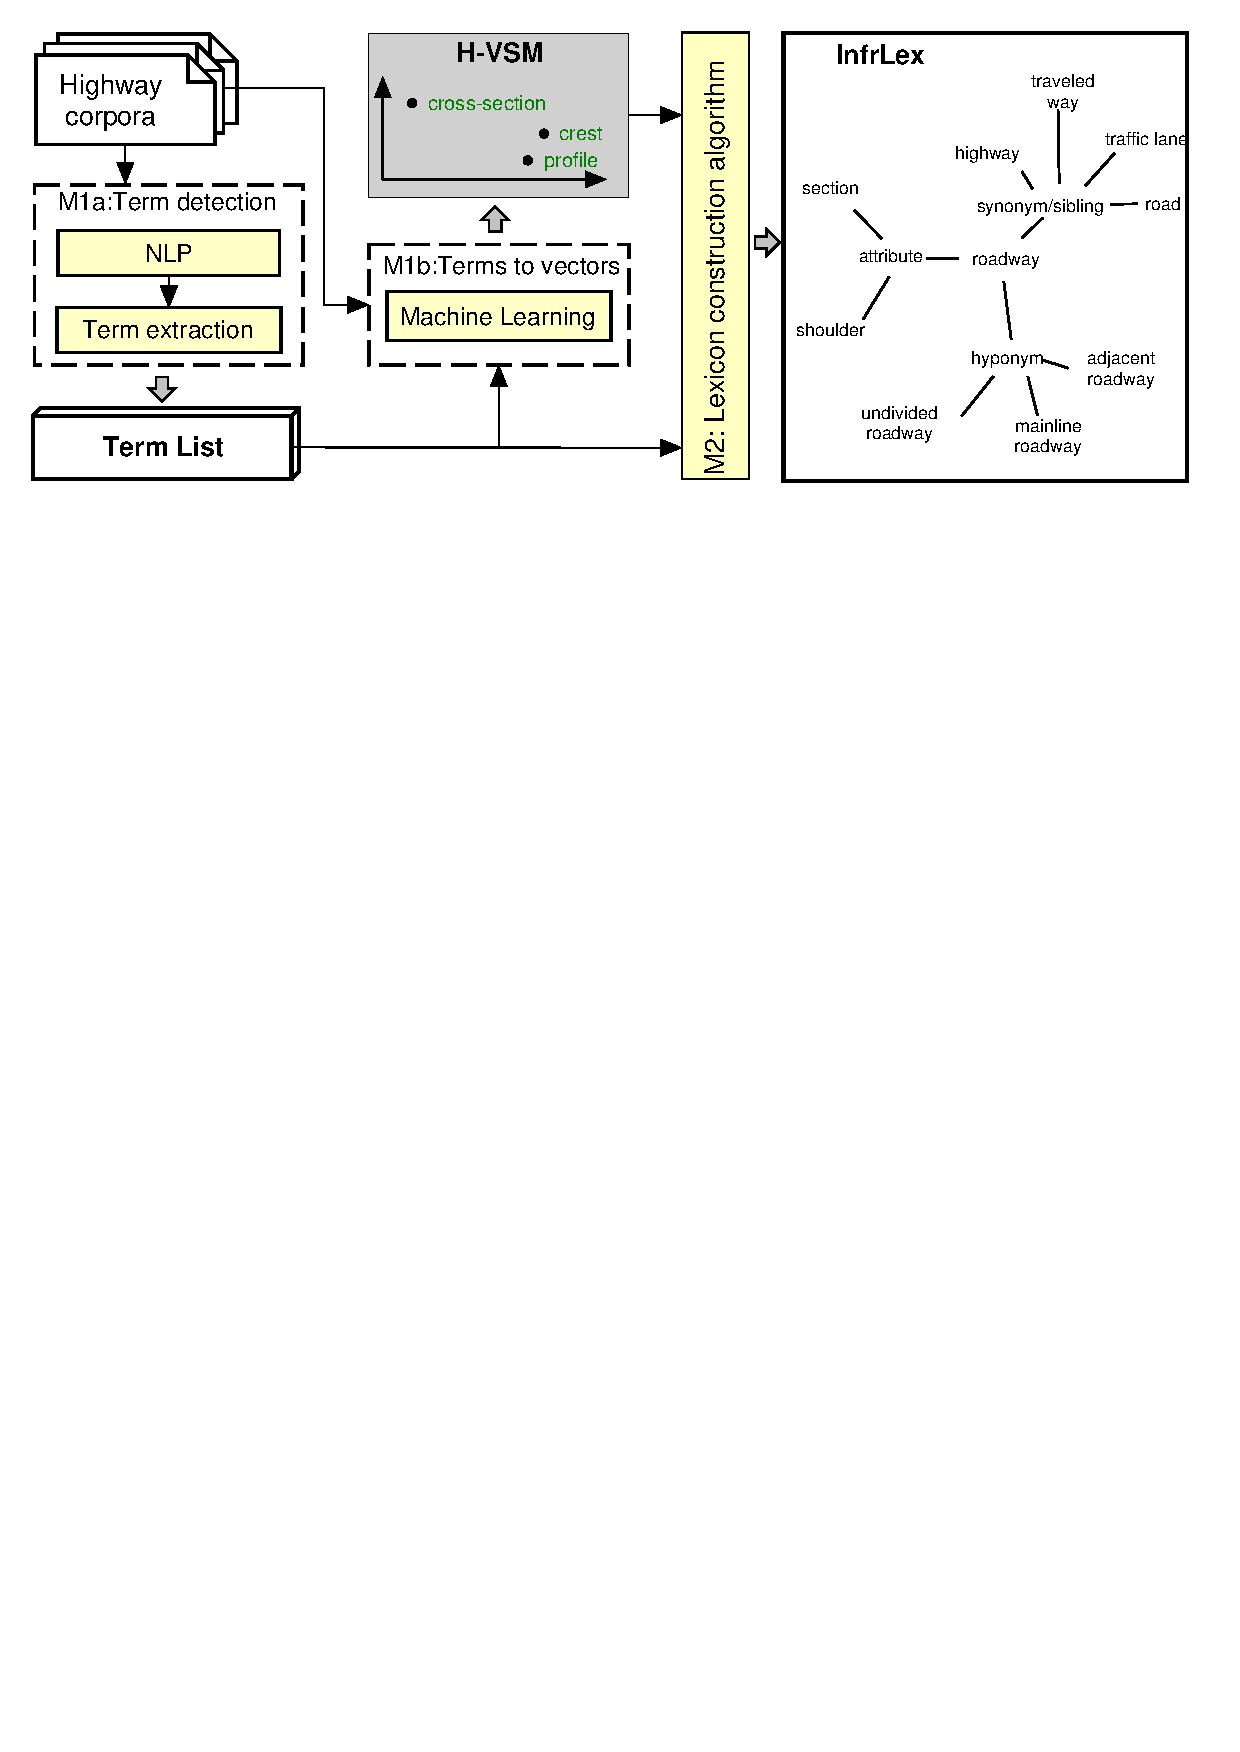
\includegraphics[width=0.95\textwidth]{proposed_methodology}
\caption{Overview of the proposed methodology}
\label{fig:framework}
\end{figure}
%
The ultimate goal of this research is to build a machine-readable dictionary of technical terms in the infrastructure sector. Conventional methods for building those dictionaries required a huge amount of empirical work, and they are still limited. Wordnet \cite{miller95} which is one of the largest lexicons available containing 117,000 synsets, but it is generic and is not suitable for the highway domain. This research propose a method for automatic construction of a domain thesaurus for the civil infrastructure sector using advanced advanced techniques of Natural Language Processing (NLP). 
\par
Figure \ref{fig:framework} presents the overview of the methodology for automated generation of a lexicon for infra structure projects (InfraLex). The research framework is consisted of two modules that are: (1) developing a highway term space model (H-VSM), and (2) InfraLex construction. The first module implements several basic NLP techniques (including tokenizing, POS tagging, etc.) and the C-value \cite{frantzi20} method to extract highway related technical concepts from the highway corpora. Skip-gram model, a unsupervised machine learning method proposed by \cite{mikolov13a}, is then implemented to train the semantic similarity between technical term using the unlabeled input data of the highway corpora. This training process transforms terms into representation vectors H-VSM.  Using this concept vector space, the degree of similarity/relatedness between technical term can be determined; and based on that the list of most semantically similar term for a given term can be obtained. In the second module, a computational algorithm is designed to classify  the nearest lists resulted from the H-VSM into lexical groups in accordance to their semantic relations such as synonymy, sibling, hypernymy, hyponymy and attribute. The following sections respectively presents the process of building the highway term space model and the searching algorithm along with details on which methods/tools utilized. 
%
%TODO: The preliminary result is presented by. In this paper, the model is extended with larger training datasets and post-processing to reorganize terms in categories which improves the semantic data searching algorithm.
%\section{Highway term space model development} \label{sec:vector-space}
%
%introduction to the distributional vector model, fundamental theory,  the overall process to translate technical terms into vectors representations. the role of vector space allow measure the similarity between 
%TODO: This section presents the extension of the H-VSM developed by the authors' previous work with the extending of training datasets and post-processing of the vector space model.

The process of developing the H-VSM includes the following steps: (1) text document collection, (2) multi-word terms extraction, and (3) semantic similarity training. The sub-sections below discuss the detailed procedures for each step. 
%
\subsection{Data collection}
%how to collect data, how to clean data to get them readay for training model
%aim text folow remained, flow direction. bottom down, 
%remove heading (chapter, section, subsection), footnote, numerbing, bullets, hyperlink, url, 
As mentioned earlier, the H-VSM was trained using a machine learning model which uses text corpus as the training data. A highway corpus was built upon the technical documents collected from multiple sources including textbooks, and highway engineering manuals from the Federal Department of Transportation (DOT) and from 22 distinct State DOTs. The focus of the highway corpora in this research is on the following three project phases: (1) design, (2) construction and (3) asset management. Technical terms in a guidance document in the engineering field are organized in various formats such as plain text, tables, and equations. Since tables and equations are not yet supported by the state-of-the-art NLP techniques, they were removed from the text corpora. The result of data collection is a plain text corpora consisting of 16 million words. This dataset is utilized to extract highway related technical terms which are then trained and converted into vectors.
%
\subsection{Multi-word terms extraction}
%
\begin{figure}[t]
\centering
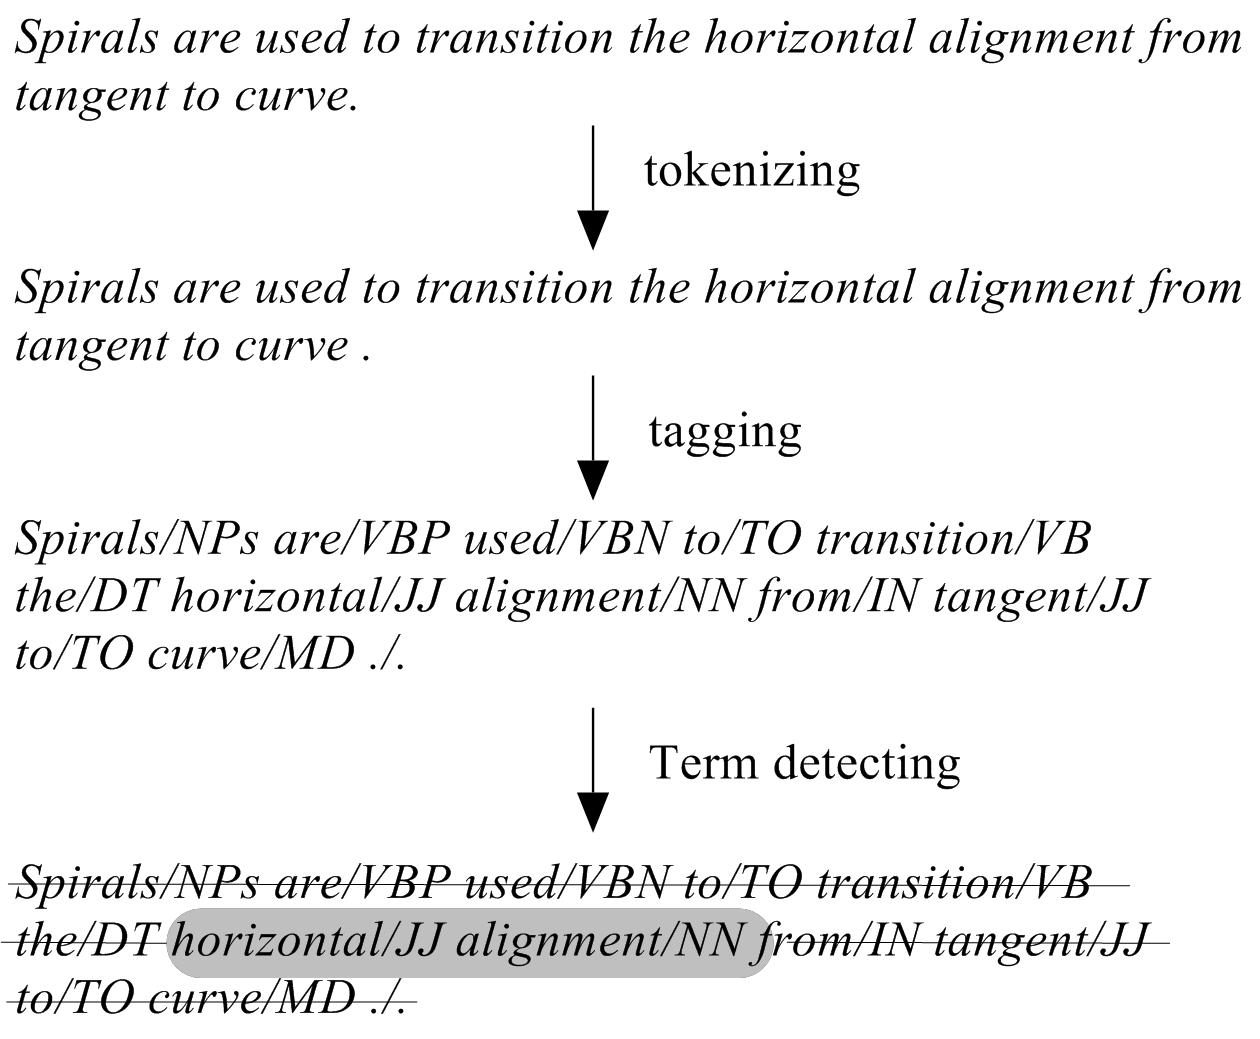
\includegraphics[width=0.45\textwidth]{NP_detecting}
\caption{Linguistic processing procedure to detect technical terms}
\label{fig:np_detect}
\end{figure}
%
A technical term can be a single word (e.g., roadway, lane, etc.) or be composed of multiple words (e.g., right of way, at grade intersection, etc.). The meaning of multi-word terms may not be directly interpreted from the meanings of their single words. In order for the Skip-gram model (in the training process) to learn the semantics of multi-word terms, the occurrence of them in the corpus need to be detected and replaced with connected blocks of word members. Figure \ref{fig:np_detect} presents the process of detecting technical terms commonly used in highway technical documents which includes the following steps. 
\par
\begin{enumerate}
	\item \textbf{Word tokenizing:} In this step, the text corpus is broken down into individual unit (also called tokens) using OpenNLP Tokenizer.
	\item \textbf{Part of Speed tagging:} The purpose of this step is to determine the part of speech tag (e.g., noun, adjective, verb, etc.) for each token.
	\item \textbf{Noun phrase detection:} Linguists argue that a technical term is either a noun (e.g., road) or a noun phrase (NP) (e.g., right of way) that frequently occurs in the domain text documents \cite{justeson95}. Thus, NPs are good multi-word term candidates. Table \ref{table:term_filter} presents the proposed extraction patterns which are modified from the filters suggested by (1995)\cite{justeson95} to extract NPs. The first two filters directly detect NPs that occur separately, and the third filter is to count for cases where multiple terms are represented in conjunctions (e.g., 'vertical and horizontal alignment'). For each instance of conjunction, an extra processing is applied to break it into individual terms. For example, the conjunction 'vertical and horizontal alignment' will become 'vertical alignment' and 'horizontal alignment'. This division process determines the main part ('alignment') which is shared by two terms and the dependent parts ('vertical' and 'horizontal'). This research use the Stanford Dependencies Parsing tool , which is able to analyze dependencies between sentiment units, to split conjunctions phrases into separate phrases. 
	%
	\begin{table} [t]
		\caption{Term candidate filters}
		\label{table:term_filter}
		\centering
		\small
		\renewcommand{\arraystretch}{1.25}
		\begin{tabular}{l l}
			\hline
			\textbf{Pattern} & \textbf{Examples}\\
			\hline
			(Adj|N)*N		& road, roadway shoulder, vertical alignment\\
			(Adj|N)*N Prep (of/in) (Adj|N)*N	&	right of way, type of roadway\\
			(Adj|N)* 'and/or' (Adj|N)*N & vertical and horizontal alignment\\
			\hline
			\multicolumn{2}{l}{\textit{Note:} |, * respectively denotes 'and/or', and 'zero or more'.  } \\
			\hline
		\end{tabular}
		\normalsize
	\end{table}
	%
	\par
	In addition, in order to avoid the distinguishing between syntactic variants of the same term, for example 'roadway' and 'roadways', term variants will be normalized. The following are three types of syntactic variants and the proposed normalization methods. 
	\begin{itemize}
		\item \textbf{Type 1} - Plural forms, for example 'roadways' and 'roadway'. The Porter stemming algorithm \cite{porter80}, which can assist the automated removal of suffixes is applied on the corpus before extracting NPs.
		\item \textbf{Type 2} - Preposition noun phrases, for example 'roadway type' and 'type of roadway'. In order to normalize this type of variant, the form with preposition needs to be converted into the non-preposition form by removing the preposition and reverse the order of the remaining portions. For example, 'type of roadway' will become 'roadway type'.
		\item \textbf{Type 3} – Abbreviations, such as AADT. A linguistic rule-based method suggested by \cite{nenadic02} will be used to determine the full term for each abbreviation. This method suggested the following abbreviation definition patterns: (1) left definition pattern – NP (Abbreviation), for example Annual Average Daily Traffic (AADT); and (2) right definition pattern - (Abbreviation) NP, for example (AADT) Annual Average Daily Traffic.
	\end{itemize}
	\item \textbf{Multi-word term candidate raking and selection:} Multi-word term definition varies between authors, and there a lack of formal rules for defining multi-word term \cite{frantzi20}.  There are a number of methods for determining termhood (the degree that a linguistic unit is a domain-technical concept) such as TF-IDF  \cite{sparck72,salton88}, C-Value \cite{frantzi20}, Termex  \cite{sclano07}. These methods are based on occurrence frequencies of NPs in the corpus. Among these methods, Termex outperformed other methods on the Wikipedia corpus, and C-Value was the best on the GENIA medical corpus \cite{zhang08}. This result indicates that C-value method is more suitable for term extraction from a domain corpus rather than a generic corpus. For this reason, the C-value has been widely used to extract domain terms in the biomedical field \cite{ananiadou20}, \cite{lossio13}, and \cite{nenadic02}). Since the corpus used in this research will be mainly collected from technical domain documents, thus C-value would be the most suitable for termhood determination. The C-value measure, as formulated in Equation \ref{eq:cvalue}, suggests that the longer a noun phrase is, the more likely that is a term; and the more frequently it appears in the domain corpus, the more likely it will be a domain term.
	% 
	\begin{equation}
	C-value(a)=
	\begin{cases}
	log_2|a|.f(a), & \text{if a is not nested} \\
	log_2|a|(f(a)-\frac{1}{P(T_a)}\sum_{b\in T_a} f(b)), & \text{otherwise}
	\end{cases}
	\label{eq:cvalue}
	\end{equation}
	%
	Where:
	\begin{description}
		\item[a] is a candidate noun phrase
		\item[f] is the frequency of a in the corpus
		\item[Ta] is the set of extracted noun phrases that contains a
		\item[P(Ta)] is the number of these candidate terms.
	\end{description}
\end{enumerate}
%
\par
The final ranked list of terms obtained which have C-value greater than 0 was manually evaluated to remove non-terms. Table \ref{table:term_evaluation} shows the evaluation result for 5 of the extracted terms. The longer the list is, the more effort required for the evaluation process. Since the the term extraction is based on frequency, the size of term list will be affected if a threshold of frequency is used. With the threshold of 2, the list consists of 112024  terms, and the the list size drops to 8922 when a threshold of 50 is used. Manually reviewing evaluate such a along list is still a challenging task. To minimize human force, the list was evaluated at several ranges of C-values. Precision, which represent percentage of real terms in each group were determined. The results are presented in Figure \ref{fig:term_precision}. As show in the figure, precision are relative low for groups with c-values less than 70. To balance between human cost and precision, this research proposes to manually review all the automatically extracted term below the c-value threshold of 70.
%To calculate the recall value, expert is required to final all true terms from the corpus \cite{frantzi20}. with the large corpus in this research, it is impossible to do this task. 
%
\begin{table} [t]
	\caption{Examples of extracted terms and evaluation}
	\label{table:term_evaluation}
	\centering
	\small
	\renewcommand{\arraystretch}{1.25}
	\begin{tabular}{l l l}
		\hline
		\textbf{Term} & \textbf{Termhood} & \textbf{real term?}\\
		\hline
		sight distance		& 9435.314 & yes\\
		design speed & 9052.556 & yes \\
		additional information & 1829.0 & no\\
		typical section & 1801.0  & yes\\
		basis of payment & 1762.478 & no\\
		\hline
	\end{tabular}
	
	\normalsize
\end{table}

\begin{figure}[t]
	\centering
	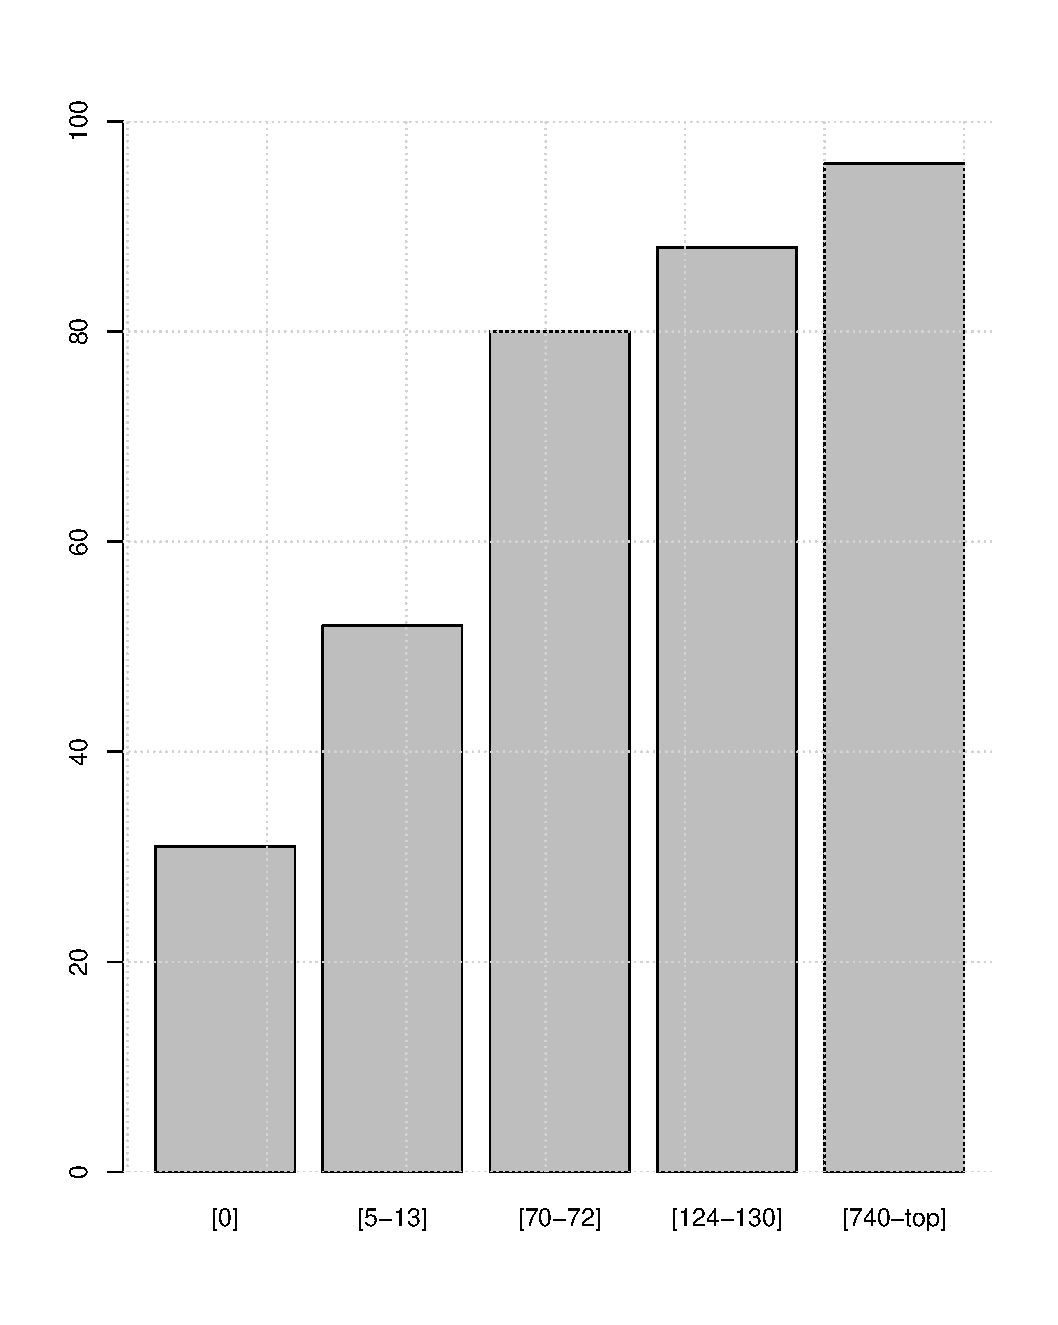
\includegraphics[width=0.5\textwidth]{term_extraction_precision}
	\caption{Precision of term extraction}
	\label{fig:term_precision}
\end{figure}

\subsection{Training dataset preparation}
The highway text copora collected serves as the source of training dataset for developing the semantic similarity model. The Skip-Gram model requires a set of training data in which the input data is a linguistic unit (word or term) and the output data is a set of context words. In order to collect this training dataset, the unannotated text corpora will be scanned to collect instances of terms and their corresponding context words. Each occurrence of a technical term will correspondingly generate a data point in the training dataset.
\par
Before collecting the training dataset, an additional step is needed to handle the issue related to multi-word terms. Since document scanning is on a word-by-word basis, the corpus must be adjusted so that multi-word terms can be treated like single words. To allow the scanner to collect both full and nested terms, any occurrence of a multi-word term in the corpus is replaced with a single unit that is compiled by connecting all individual words. For instance, ‘vertical alignment’ will become ‘vertical\_alignment’.
%
\par
The adjusted highway corpus is scanned through to find the context words for every occurrence of the technical terms in the vocabulary. The number of context words to be collected is dependent on the window size that limits how many words to the left and to the right of the target word. In the example sentence below, the context of the term 'roadway' with the context window size 10 will be the following word set {bike, lane, width, on, a, width, no, curb, gutter}. Any word in the stop list (a list of frequent words in English such as 'a', 'an', 'the' that have little meaning) will be neglected in the context set. If the target word is a multi-word term, the set of context words will not include its member words. 
%
\begin{center}
	"The minimum [bike lane width on a roadway with no curb and gutter] is 4 feet."
\end{center}
%
\subsection{Semantic similarity training}
%word2vec, brief introduction about word2vec
%skip-gram model
%how to modify the method of selecting conext words
%java program

\begin{figure}[t]
	\centering
	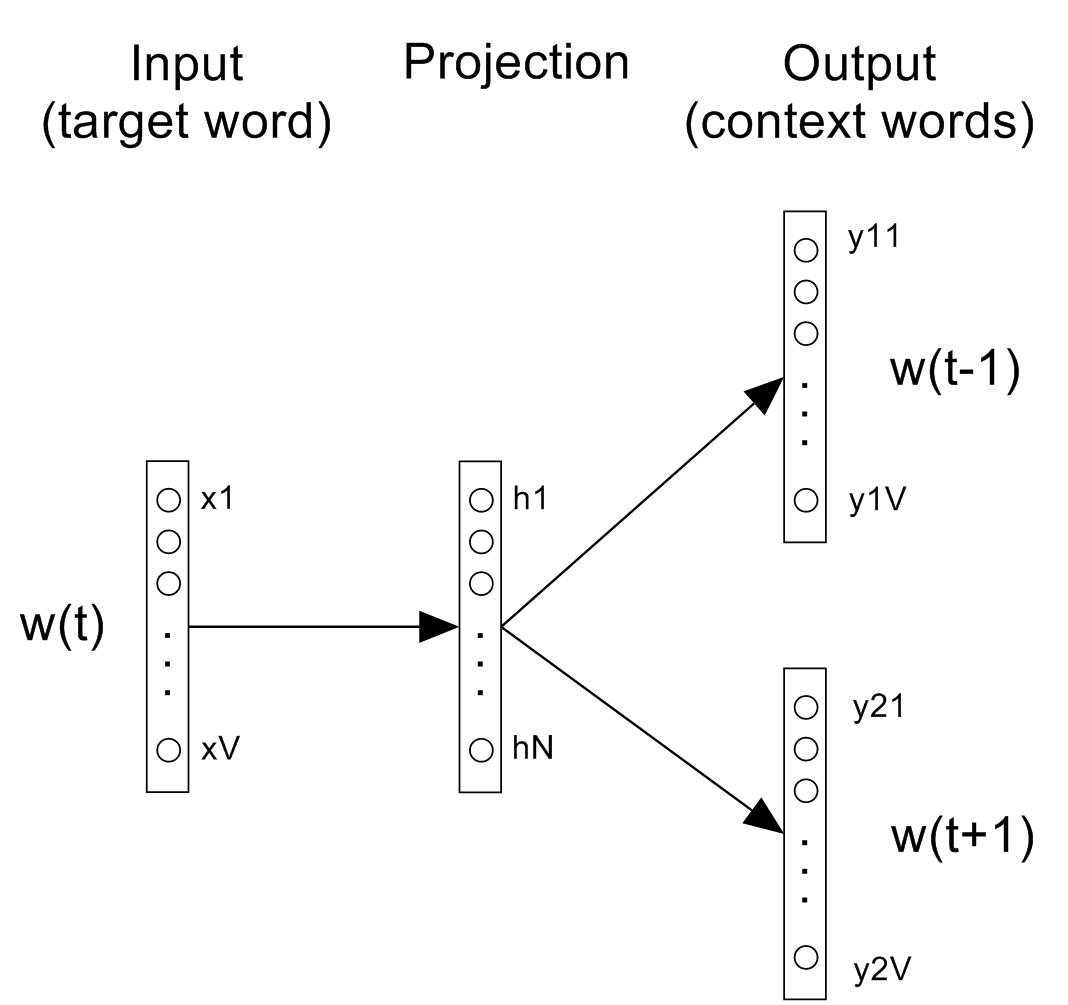
\includegraphics[width=0.45\textwidth]{skip-gram-model}
	\caption{Skip-gram model}
	\label{fig:skip-gram}
\end{figure}

The semantic similarity will be trained using the word2vec module in the Apache Spark MLlib package \cite{apache16}, an emerging open-source engine, developed based on the Skip-gram neural network model (Mikolov et al. 2013) \cite{mikolov13a}. The intended parameters used for the training model are presented in Table \ref{table:nn-parameters}. These values are mainly based on suggestions from the literature. To eliminate data points with low frequency of occurrence that are unlikely to be technical terms, word2vec includes the parameter of minimum occurrence frequency. Any vocabulary with the rate lower than the limit will be ignored. Radim Rehurek, a machine learning consultant company, suggests a range of (0-100)* depending on the data set size. Setting this parameter high will enhance the accuracy, but many technical terms will be out of vocabulary. The preliminary study based on the preliminary corpus with only several millions of words shows that with the frequency of 20, there are very few non-technical terms involved in the training dataset. Hence, with the larger dataset to be collected, this parameter can be higher and up to around 50. The second important parameter is layer size which determines the number of nodes in the hidden layer. This parameter highly affects the training accuracy and processing time. A larger layer size is better in terms of accuracy but this will be paid off by the running time. Since this research aims to develop a model that can be used for other information retrieval research, the accuracy is the first priority. This parameter may range from 10 to hundreds; in this research, it is expected to in be the range of 100-500. The final major parameter is the context window size. Google  suggests the size of 10 for the Skip-gram model. These parameters are subject to be changed so that the best model can be achieved. The effects of these parameters to the performance of the synonym detection application are discussed in Section \ref{sec:eval}.
%
\begin{table} [t]
\caption{Skip-gram model parameters}
\label{table:nn-parameters}
\centering
\small
\renewcommand{\arraystretch}{1.25}
\begin{tabular}{l l}
\hline
\textbf{Parameter} & \textbf{Value}\\
\hline
Frequency threshold & 50-100\\
Hidden layer size		&	100-500\\
Context window size	&	5,10,15\\
\hline
\end{tabular}
\normalsize
\end{table}
%
Figure \ref{fig:hvsm} presents the term space model developed from the training process with the parameters are 50, 300 and 10 respectively. In this model, each technical term collected from technical documents is represented as a vector in a high dimensional space; and the distance between them represents the semantic similarity. The preliminary term space presented in this paper consists of more than six thousand technical keywords. Since the vector space is a multi-dimensional space according to the size of hidden layer. In order to illustrate, present space in 2D graph, PCA (Principle component Analysis) was used to reduce the size to 2 dimensions. The similarity between terms can be measured by the angle between two work representation vectors or the distance between two word points. The following shows two measures of word sense similarity. Table \ref{table:nearest_example} shows an ranked list of near terms obtained from the H-VSM model.
%
\begin{figure}[t]
	\centering
	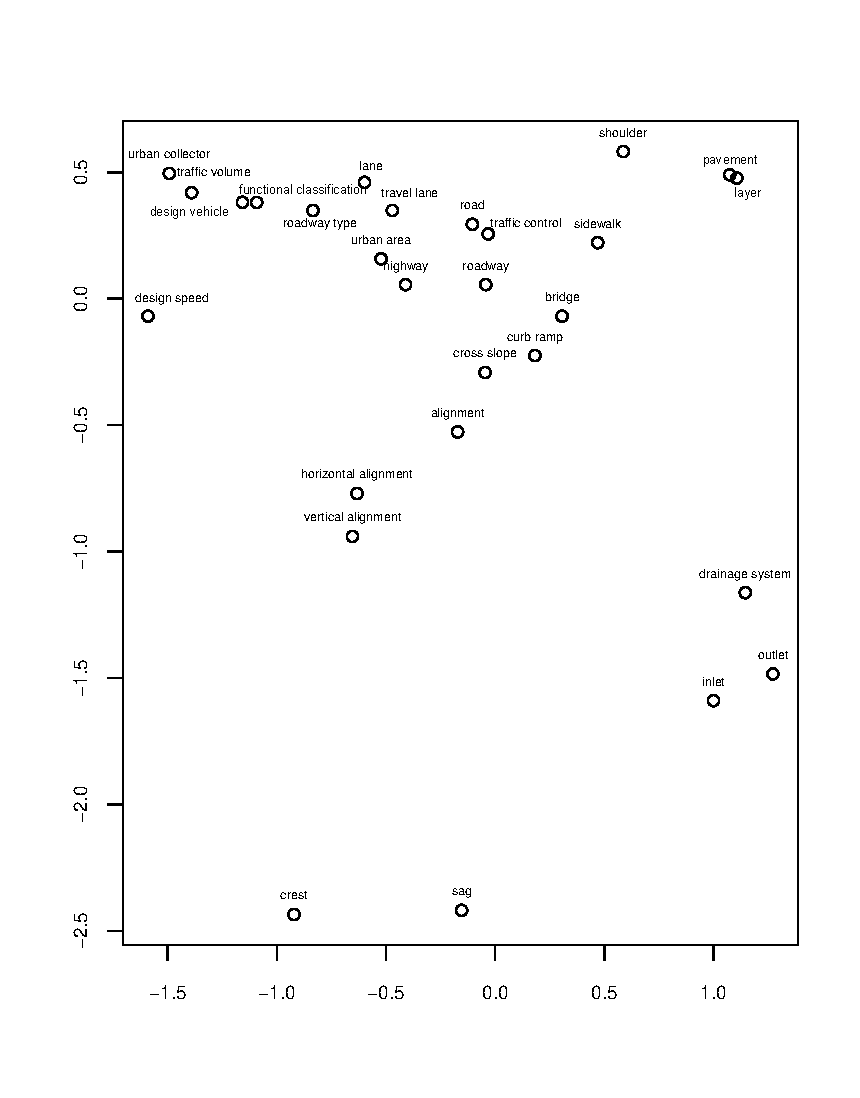
\includegraphics[width=0.45\textwidth]{Rplot_space}
	\caption{Highway term space model (H-VSM)}
	\label{fig:hvsm}
\end{figure}
%
\begin{equation}
cosine\_similarity = \frac{A.B}{||A||.||B||}
\end{equation}

\begin{equation}
dis\_similarity =\sqrt{(xA_1-xB_1)^2+(xA_2-xB_2)^2+...+(xA_n-xB_n)^2}
\end{equation}

Where: n is the hidden layer size.
%
\begin{table} [t]
	\caption{Examples of top nearest terms}
	\label{table:nearest_example}
	\centering
	\small
	\renewcommand{\arraystretch}{1.25}
	\begin{tabular}{l l l  l}
		\hline
		\textbf{Term} & \textbf{Nearests} & \textbf{Cosine} &\textbf{Rank}\\
		\hline
		roadway			& highway & 0.588 & 1\\
						& traveled-way & 0.583 & 2\\
						& roadway-section & 0.577 & 3\\
						& road & 0.533 & 4\\
						& traffic-lane & 0.524 &5\\
						& separating & 0.522 &6\\
						& adjacent-roadway & 0.519 & 7\\
						& travel-way & 0.517 & 8\\
						& entire-roadway & 0.513 & 9\\
						& ...&...& ...\\
						& roadway-shoulder & 0.505 & 12\\
						& roadway-cross-section & 0.491 & 18\\
						& undivided & 0.452 & 37\\
						& mainline-roadway & 0.450 & 42\\
		\hline
	\end{tabular}
	\normalsize
\end{table}

\subsection{Highway lexicon construction}
The purpose of this module is to construct a lexicon which is also known as lightweight ontology. A knowledge base typically includes terms and relations. The core relations of an ontology can be classified into the following types: synonym (meaning equivalence), hypernym-hyponym (also known as IS-A or parent-child relation), attribute (concept property), and association (e.g. part-of) \cite{jiang97,lee13}. If two terms relate each other through these semantic relation would have high similarity. Therefore, the top nearest terms resulted from H-VSM would be a great starting point for detecting relations between technical terms. Table \ref{table:nearest_example} illustrates a list of nearest terms of the term 'roadway'. In this list, true synonyms are highway (1), traveled-way (2) or road(4); roadway-section (3), roadway-shoulder (12) are attributes of the roadway concept; and adjacent-roadway (7), undivided (37) are hyponyms which showing different types of roadway.
\par
The specific objective of this task is to detect relations and based on that rearrange the vocabulary constructed in the first module. Algorithm \ref{alg:term_class} shows the design pseudo code for classify the nearest terms of a given target term. The algorithm utilizes linguistic rules and clustering analysis to reorganize the nearest list into the following three groups including (1) attribute, (2) hyponym and (3) synonym/sibling and functional relation. The algorithm firstly detects terms for the first two categories using linguistic rules. The filter rules to detect these relations are presented in Table 3. For example, with pattern 1, we can infer that Noun1 is a good attribute candidate of concept Noun2; and Noun2 is an attribute of Noun1 in the pattern 2. The remained words will fall into the third group. However, some of them have far or even no relation with the target word. In order to address this issue, this research employed the K-mean clustering algorithm \cite{macqueen67} to split the remained list into three distinct layers based on their similarity score. The terms in the last group are unlikely to be a synonym or sibling and is removed from the nearest list. The outcome of the proposed algorithm is a list of classified nearest term. Table \ref{table:term_clustering} shows one example for the output retrieved from the algorithm. 
%In contrast, since synonym recognition is well known as the process of evaluating the sharing of common attributes, hypernyms, and hyponyms, this process will rely on the results from the detection of other relations. This task will first detect the following relations (hypernyms, hyponyms and attributes) and then use them as features to find synonyms.
%
\begin{algorithm}
	
	\caption{Near term classification algorithm}\label{alg:term_class}
	\begin{algorithmic}[1]
		\State \textbf{Inputs}: term \textit{t}, list of nearest terms \textit{N}, full list of terms \textit{F}
		\State \textbf{Output:}: Classified list of terms \textit{C}
		\Procedure{Term classification procedure}{}
		%\State $\textit{n} \gets \text{size of }\textit{W}$
		%\State $\textit{m} \gets \text{size of }\textit{T}$
		\State $\textit{Att} \gets \text{list of attributes}$
		\State $\textit{Hyp} \gets \text{list of hyponyms}$
		\State $\textit{Syn} \gets \text{list of synonyms}$
		\State $\textit{w} \gets \textit{null}$
		\ForAll {$n \in N$}
			\If {$n$ contains \textit{t}}
				\State $w \gets n$
	
			\Else
				\ForAll {$f \in F$}
					\If {$f$ contains both $n$ and \textit{t}}
						\State $w \gets f$	
						\State Break for

					\EndIf
				\EndFor
			\EndIf
		\EndFor
		\If {$w$ matches \textit{Attribute pattern}}
			\State add $w$ to \textit{Att}
		\ElsIf {$w$ matches \textit{Hyponym pattern}}
			\State add $w$ to \textit{Hyp}
		\Else
			\State add $w$ to \textit{Syn}
		\EndIf
		\State Cluster \textit{Syn} and discard low relevant terms

		\EndProcedure
	\end{algorithmic}
\end{algorithm}
%
%\subsection{Attribute and hyponym patterns}
%
\begin{table} [t]
	\caption{Patters to extract attributes and hyponyms}
	\label{table:attribute_pattern}
	\centering
	\small
	\renewcommand{\arraystretch}{1.25}
	\begin{tabular}{l l l}
		\hline
		\textbf{Relation} \textbf{Pattern} & \textbf{Example}\\
		\hline
		Attribute &	Noun of Target & the width of the road\\
		& Target Noun	&	road width, project cost\\
		Hypernym-hyponym & Noun Target & vertical alignment isA alignment\\
		\hline
	\end{tabular}
	\normalsize
\end{table}
%
%After the candidate list is refined, the frequency of occurrence for each candidate will then be used to compute the degree that term 'a' is an attribute of concept 'c'. If 'a' is a typical attribute of 'c', it should frequently occur in the corpus. Each concept 'c' will correspondingly have a list of attribute candidates (called list A) and their frequency of occurrences. The likelihood that 'a' is an attribute of concept 'c' is estimated using the normalized probability formula (see Equation \ref{eq:attribute}). The attribute candidates for each concept will be ranked by the likelihood measure and the top list over a threshold value will be accepted as typical attributes. 
%\begin{equation}
%P(a|c)=\frac{n(c,a)}{\sum_{a* \in A} n(c,a)}
%\label{eq:attribute}
%\end{equation}
%\subsection{Synonym/sibling and functional relation recognition}

%
\begin{table} [t]
	\caption{Examples of top nearest terms}
	\label{table:term_clustering}
	\centering
	\small
	\renewcommand{\arraystretch}{1.25}
	\begin{tabular}{l l l l l}
		\hline
		\textbf{Term}	&\textbf{Relation Group}	& \textbf{Nearests} & \textbf{Cosine} & \textbf{Rank}\\
		roadway			&Synonym					& highway & 0.588 & 1\\
						&							& traveled-way & 0.583 & 2\\
						&							& road & 0.533 & 4\\						
						&							& traffic-lane & 0.524 &5\\ 						
						&							& travel-way & 0.517 & 8\\  \cmidrule{2-5}
						&Attribute					& separating & 0.522 &6\\
						&							& roadway-section & 0.577 & 3\\						
						&							& roadway-shoulder & 0.505 & 12\\
						&							& roadway-cross-section & 0.491 & 18\\\cmidrule{2-5}						
						&Hyponym					& adjacent-roadway & 0.519 & 7\\
						&							& entire-roadway & 0.513 & 9\\
						&							& undivided & 0.452 & 37\\
						&							& mainline-roadway & 0.450 & 42\\
		\hline
	\end{tabular}
	\normalsize
\end{table}


\section{Performance evaluation} \label{sec:eval}
%evaluation method
This section presents the performance evaluation of InfraLex in terms of supporting identifying synonyms. In regard of the performance on synonym searching, a gold standard  is used. The gold standard is consisting 70 sets of synonyms (both single and multi-word terms) which is examined and extracted from a Wikipedia transportation glossary \cite{wikipedia16}. This glossary provided plain text explanation for each term and their synonyms. The automatically identified synonyms which are the top nearest words in the identified synonym lists from the algorithm were compared with the true synonyms in the gold standard dataset. The results are measured using the following three measures including recall, precision and f-measure.
%
\begin{align} 
&Recall = \frac{\text{number of correctly matched concepts}}{\text{total concepts}}  \\ 
&Precision = \frac{\text{number of correctly matched concepts}}{\text{total matched concepts}}  \\
&F-measure = \frac{2.Precision.Recall}{Precision+Recall}
\end{align}
%results
\begin{table} [b] 
	\caption{Effects of training parameters on performance of synonym matching}
	\label{table:eval_syn_par_effect}
	\centering
	\small
	\renewcommand{\arraystretch}{1.25}
	\begin{tabular}{l l l l l }
		\hline
		\hline
		\textbf{Parameter} & \textbf{Model} & \textbf{Precision (\%)}  & \textbf{Recall(\%)} & \textbf{F (\%)}\\
		\hline
		Baseline	&	50-100-5	&79		&53		&63\\
		\hline
		\textbf{Window size}	&\textbf{50-100-\underline{10}}	&\textbf{81}		&\textbf{54}		&\textbf{65}\\
					&50-100-\underline{15}	&81		&54		&65\\
		\hline		
		Frequency threshold	&\underline{75}-100-5	&74		&50		&60\\
							&\underline{100}-100-5	&77		&51		&62\\
		\hline
		Hidden layer size	&50-\underline{200}-5	&79		&53		&63\\
		\hline
		\hline
	\end{tabular}
	\normalsize
\end{table}
\par
%synonym matching peformance result
Table \ref{table:eval_syn_par_effect} shows the performance with different training model settings. The baseline model parameter are set 50, 100 and 5 respectively for frequency threshold, hidden layer size and window size. We changed these parameters one by one and remained the other ones to evaluate their effects to the model performance. As presented in the table, the increase of window size to 10 or 15 resulted in the best model which have precision of 81\% and an F-measure of 65\%. The change of other parameter does not improve the performance. Especially, the increase of frequency threshold have negative impact. 
%compared to the previous publication by the authors, this algorithm has been improved with significantly higher accuracy. the post-processing is one reason for the out-performance of the proposed method.  
%
%result
\begin{table} [b] 
	\caption{Comparison of synonym matching performance between Wordnet and InfraLex}
	\label{table:eval_syn_vs_Wordnet}
	\centering
	\small
	\renewcommand{\arraystretch}{1.25}
	\begin{tabular}{l l l l }
		\hline
		\hline
		\textbf{Lexicon} & \textbf{Precision (\%)}  & \textbf{Recall(\%)} & \textbf{F (\%)}\\
		\hline
		Wordnet	&76 	&40 	&52\\	
		\textbf{InfraLex} &\textbf{81}	&\textbf{54}		&\textbf{65}\\	
		\hline
		\hline
	\end{tabular}
	\normalsize
\end{table}
\par
Table \ref{table:eval_syn_vs_Wordnet} shows the comparison of performance between InfraLex (with 50-100-10 settings) and Wordnet. As shown, InfraLex outperformed Wordnet in all aspect, and the combined F-measure is significantly improved (65 compared to 52). The biggest contribution to the improvement is the recall value which represents the coverage of domain vocabulary. 
\par
Future research is till needed to enhance the performance of InfraLex, especially the recall measure. One potential reason for the low recall is due to the the training data size. This model currently is based on the data training set consisting of only 16 million words. In order to enhance the accuracy, the data training set needs to be extended in size and in the numbers of disciplines related to highway projects. 
%attribute  hyponyms and attributes. finding performance
%for attribute and hyponym only precision is determined. to determine the recall require of all possible true attributes for a concept which is challenging and unrealistic task, this research evaluate the accuracy of the extracted attributes. this largely depend on the size and the variety of discipiline covered in the corpus. select of one in each set of synonyms in the gold standard and  humam evaluate attribute and non-attribute. the performance in measure using Equation which represent the percentage of correctly extracted attribute/hyponym. 
%
\section{Discussions} \label{sec:dis}
%limitation and potential direction for improvement
the current study as a number of limitations. first, the highway corpus is till relative small with only 160 million words, compared to corpus in other domain, this is relative small. since the the recall largely depends on the corpus size. the larger corpus the more vocabulary can be extracted and larger size means some more technical terms can be covered.  
%potential application
\par
This method is broad for nlp and linguistics tools and can be applied to other business processes such as green building checking, environment checking, etc. The method is expected to significantly improve the existing ad-hoc method of model view definition development and in return leads the the removal of this bottle neck which is restricting the seamless data integration and exchange across phases of a highway construction project. Emerging of text mining and natural language processing related research. the following application can be used: (1) text mining to extract information from text of which the basic linguistic unit is term. understanding of term meaning through it's synonyms, hyponyms and attributes will allow computer to extraction information precisely.   (2) natural language interface. the current interaction between computer and user, for example in data extraction require big effort from user, a natural language interface which can understand natural language user's input will allow the automatic extraction of information. data information retrieval query by query their sysnonym, information classification. use for disambiguation task to interpret user's intention.  

\section{Conclusions} \label{sec:conclns} 
Data manipulation and retrieval from multiple sources is challenging task due to inconsistency of data format and terminology. The contribution of this study This research develops a digital dictionary of  highway related technical terms which can enable computer understand semantic meanings of terms.  this research employs advanced NLP techniques to extract technical terms from a highway text corpus cosisting of 160 million words built on design manuals from 22 State DOT across the U.S. Machine learning were used to train semantic similarity between technical terms which can be used to retrieve a list of most semantically similar terms.  A algirthm was designed to framework that semantically searches for desired data from the transferred data file. The framework is composed of two components including (1) a terms space model which represents highway related concepts extracted from the highway corpora in vectors and (2) a context based searching algorithm that can search for entities in the Landxml schema based on their similarity of attributes instead of string based similarity.
\par
The framework has been evaluated by comparing the resulted obtained from the InfraLex model and a man-crafted gold standard. The result shows the accuracy of over 80 percent.  the best model achiveed with the window size of 10. The accuracy is low due to the size of the training data. Future research will be conducted to expan the highwah corpus to further disciplines such as asset management, trasportation operation. 
\par
the research open new gate for computerational tools regarding natural lanauge processing in the highway sectors. the infraLex would enable computer to understand terms and consequently transform the way human interact with computer. once the ease of use when natural language can be used, the seamless reuse of lifecyle data would be achieved in the highway sector. 

%bibliography
\bibliography{2nd_paper_bib}
%
%
\end{document}

